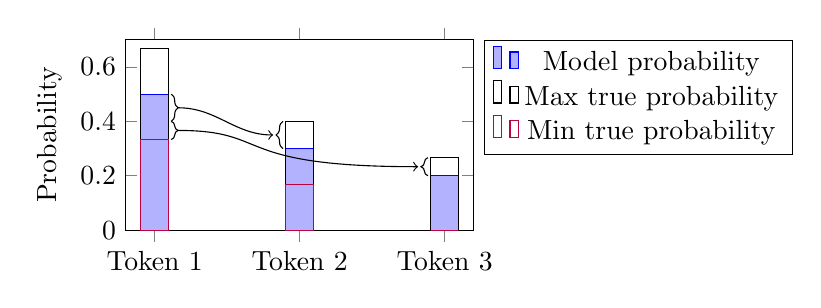
\begin{tikzpicture}
  \begin{axis}[
      ybar,
      width=6cm,
      height=4cm,
      ylabel=Probability,
      xtick distance=1,
      symbolic x coords={Token 1, Token 2, Token 3},
      ymin=0.0,
      ymax=0.7,
      legend pos=outer north east,
    ]
    \addplot+[bar shift=0pt] coordinates {
      (Token 1,0.5)(Token 2,0.3)(Token 3,0.2)
    };
    \addplot[bar shift=0pt] coordinates {
      (Token 1,0.6667) (Token 2, 0.4) (Token 3, 0.2667)
    };
    \addplot[color=purple, bar shift=0pt] coordinates {
      (Token 1,0.3333) (Token 2, 0.1667) (Token 3, 0.0)
    };
    \legend{Model probability, Max true probability, Min true probability}

    \draw[
      decoration={brace,raise=6pt},decorate
    ] (axis cs:Token 1, 0.5) -- node (a) {} (axis cs:Token 1, 0.4);
    \draw[
      decoration={brace,mirror,raise=6pt},decorate
    ] (axis cs:Token 2, 0.4) -- node (b) {} (axis cs:Token 2, 0.3);
    \draw[->] ([xshift=5pt]a.east) to[out=east, in=west] ([xshift=-6pt]b.west);

    \draw[
      decoration={brace,raise=6pt},decorate
    ] (axis cs:Token 1, 0.4) -- node (a) {} (axis cs:Token 1, 0.3333);
    \draw[
      decoration={brace,mirror,raise=6pt},decorate
    ] (axis cs:Token 3, 0.2667) -- node (b) {} (axis cs:Token 3, 0.2);
    \draw[->] ([xshift=5pt]a.east) to[out=east, in=west, in looseness=2] ([xshift=-6pt]b.west);

  \end{axis}
\end{tikzpicture}
